\section{User Interface}
\label{design:ui}

In this section, a design of wireframes will be discussed.

\subsection{Sign In and Sign Up Screens}

\begin{figure}
    \centering
    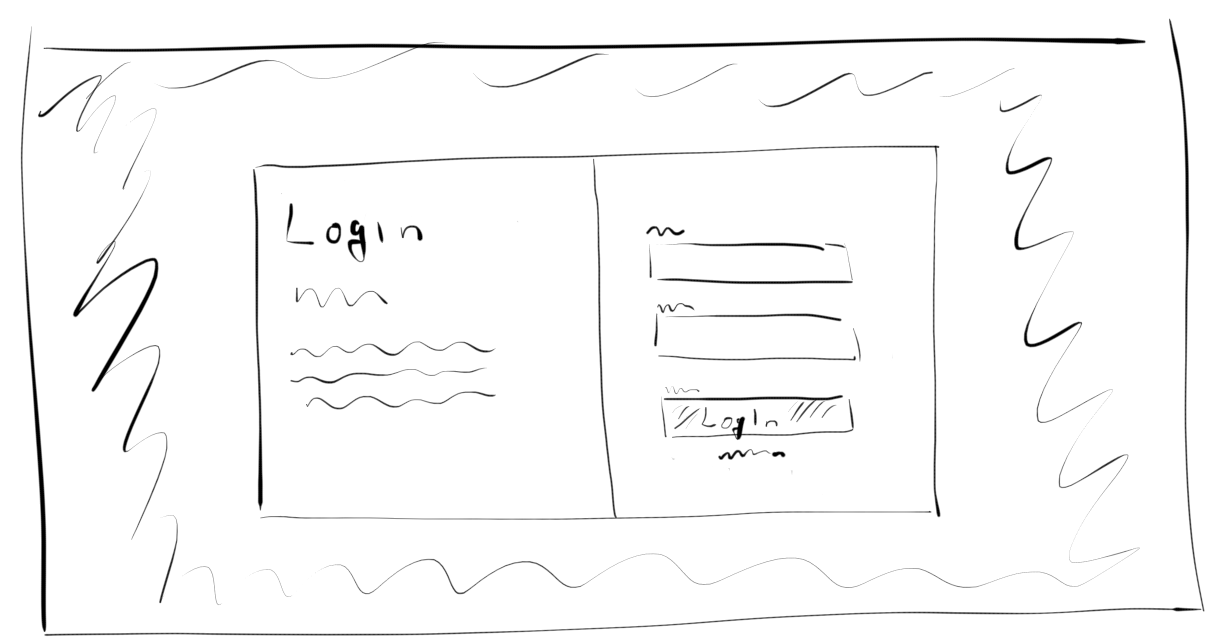
\includegraphics[width=1\linewidth]{assets/design/ui/wir_login.png}
    \caption{Sign In Wireframe}
    \label{fig:design:wir:login}
\end{figure}

On the screen, \ref{fig:design:wir:login} will be one of the important components -- sign in and sign up.
If the user does not register or log in, he cannot play the game.
Therefore, it will be more than appropriate if the screen is simple and contains a meaningful design.

The screen contains text inputs for entering nicknames, passwords, and more and includes a button that is used to submit the form.

\subsection{Missions Screen}

Missions screen \ref{fig:design:wir:missions} is a transition screen for selecting missions to play.
It contains a top menu from which it is possible to access all stories, statistics, a profile, and a button on the main page.

It contains an overview of individual missions, tuned into a linear sequence, but it is also possible to make a divided linear sequence of missions.
A line is displayed between the missions, indicating continuing to the next mission.
Next to the mission is its name.

\begin{figure}
    \centering
    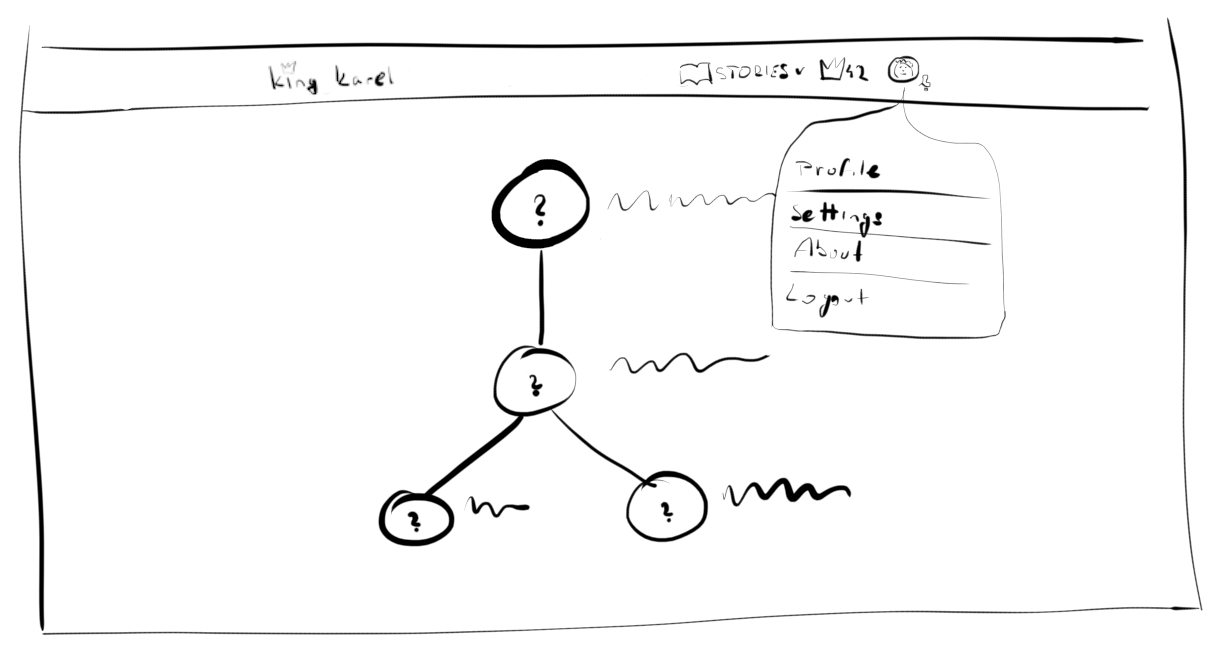
\includegraphics[width=1\linewidth]{assets/design/ui/wir_stories.png}
    \caption{Missions Wireframe}
    \label{fig:design:wir:missions}
\end{figure}

\subsection{Story Screen -- Game}

Story screen with click on a game mission on figure \ref{fig:design:wir:story-game}.
The click will show a bubble dialog that contains information about the number of points completed, the mission name, the caption, and the play button.

\begin{figure}
    \centering
    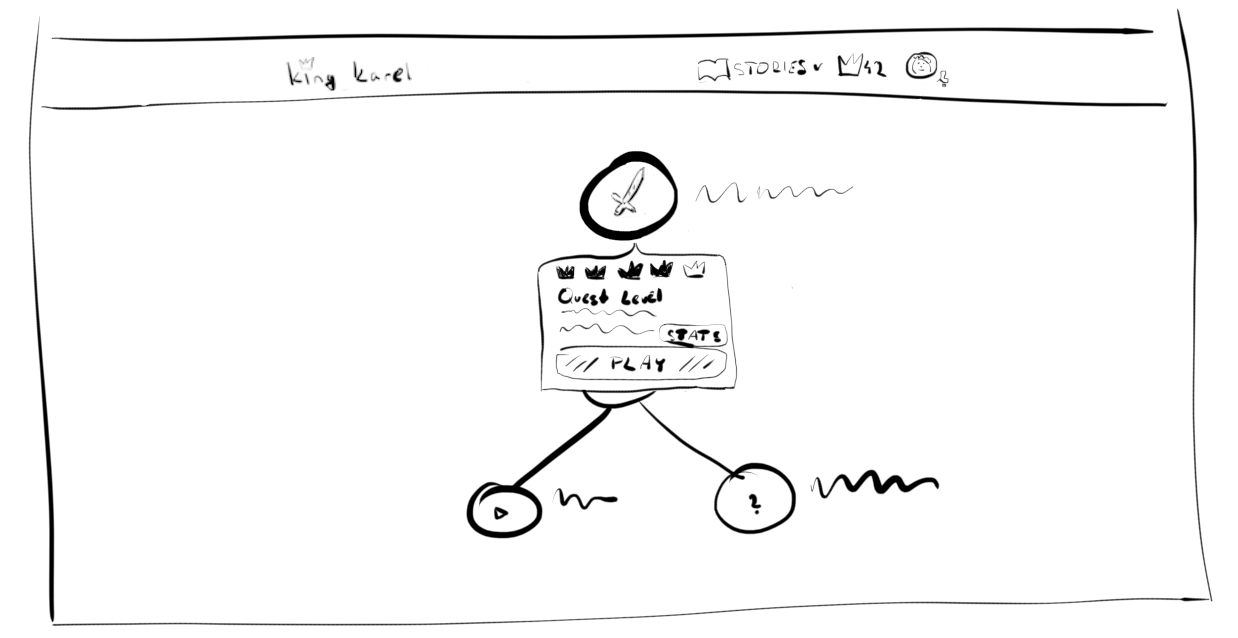
\includegraphics[width=1\linewidth]{assets/design/ui/wir_game.png}
    \caption{Game Mission Wireframe}
    \label{fig:design:wir:story-game}
\end{figure}

\subsection{Story Screen -- Learning and Storytelling}

Like the previous wireframe, on figure \ref{fig:design:wir:story-learning} there is a story screen which, after clicking on the learning mission or storytelling mission, displays a bubble dialog with information about the learning mission or storytelling mission.
It contains information about the title, description, and a button to start a learning or storytelling mission.

\begin{figure}
    \centering
    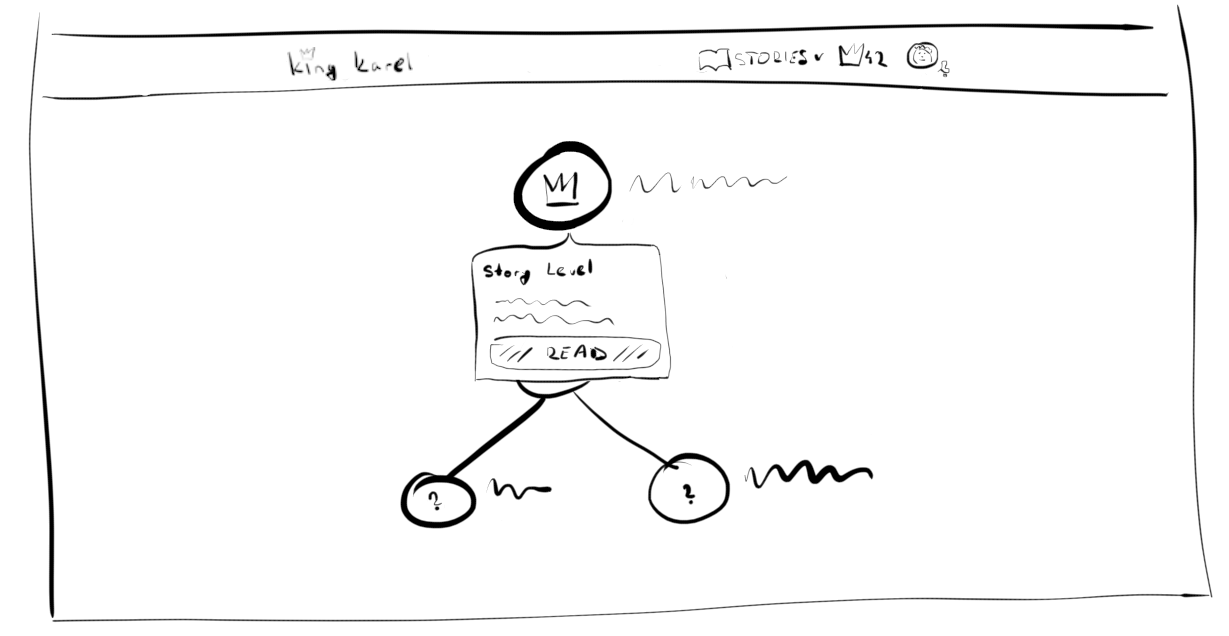
\includegraphics[width=1\linewidth]{assets/design/ui/wir_story.png}
    \caption{Learning and Storytelling Missions Wireframe}
    \label{fig:design:wir:story-learning}
\end{figure}

\subsection{Game Mission Screen}

The main part of the prototype of the developed game is on the screen \ref{fig:design:wir:game-mission}.
It contains both a top menu that includes buttons to jump to the main screen, stories, statistics, and a profile.

The screen contains a panel with command blocks on the left.
These are arranged below each other and possibly nested inside each other.
To the right of this is a palette of commands that can be used for a given mission.

Below these panels, there is no panel at the bottom with buttons to save and stop the game.

In the right part of the screen, there is a grid display that represents the game's current state.
The grid can display walkable lungs or non-walkable squares that form walls or other types of obstacles.
The grid also shows a doll that marks the robot, Karel.
That is the character the player is playing as.

\begin{figure}
    \centering
    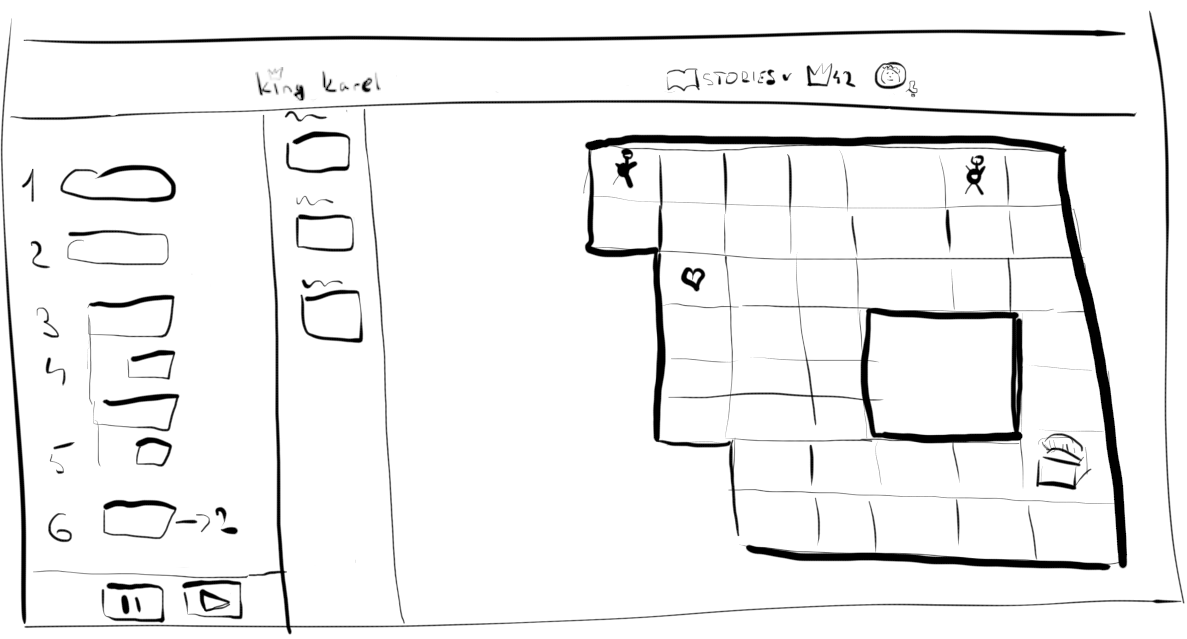
\includegraphics[width=1\linewidth]{assets/design/ui/wir_game_mission.png}
    \caption{Game Mission Wireframe}
    \label{fig:design:wir:game-mission}
\end{figure}

\subsection{Game Dialog}

At the end of the game, whether successful or not, a \ref{fig:design:wir:game-dialog} dialog window will appear with a status message.
This dialog reports whether the game ended with an error or successfully.
In addition, the dialog contains a caption.
The optional size and speed bonus attributes are displayed if the status is successful.

\begin{figure}
    \centering
    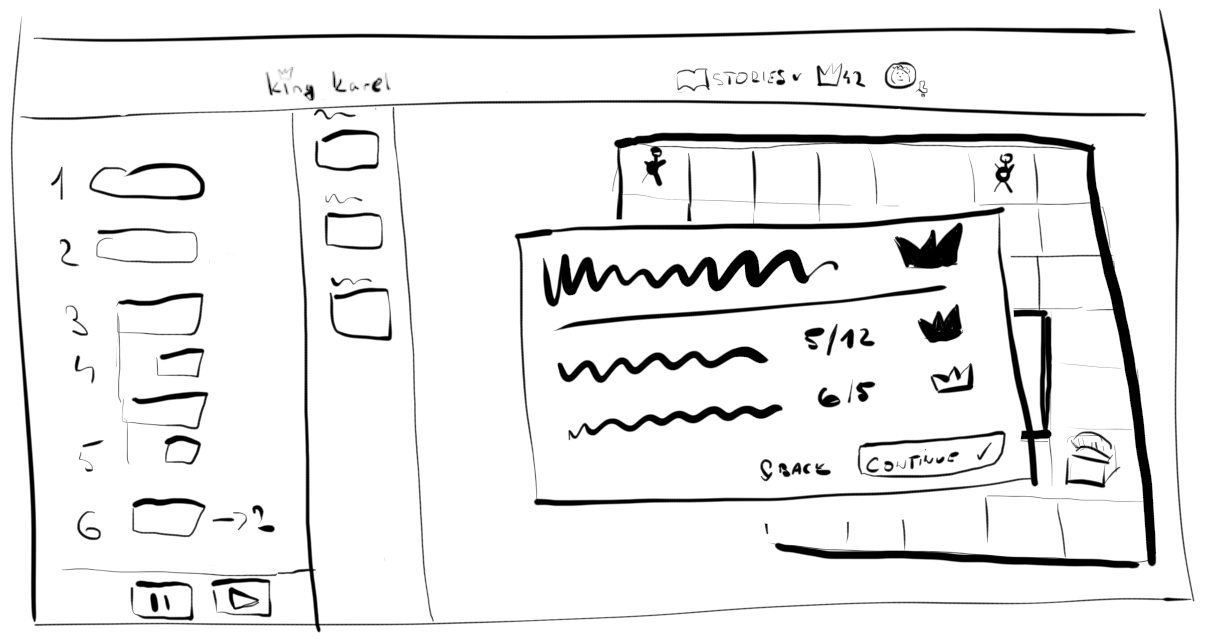
\includegraphics[width=1\linewidth]{assets/design/ui/wir_game_dialog.png}
    \caption{Game Mission Dialog Wireframe}
    \label{fig:design:wir:game-dialog}
\end{figure}

\subsection{Statistics Screen}

The statistics screen \ref{fig:design:wir:statistics} shows the status of success of game missions and values of the optional size and speed attributes.
It displays it in the tabular form separately according to yourself and other players.
The statistics are divided according to the game mission.

\begin{figure}
    \centering
    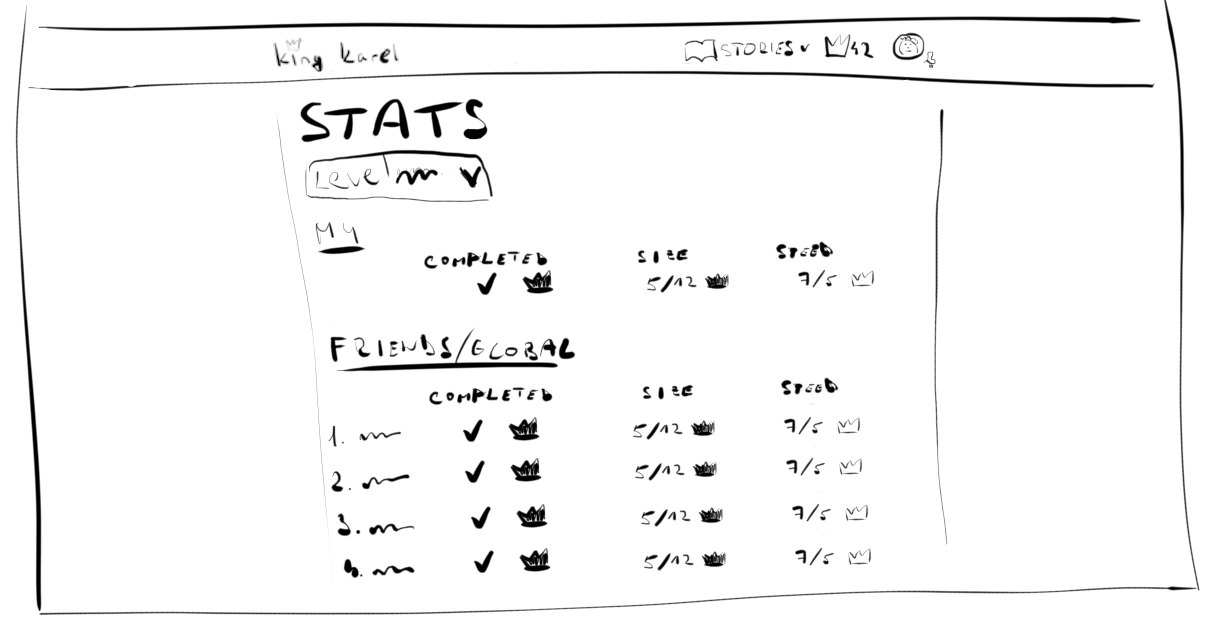
\includegraphics[width=1\linewidth]{assets/design/ui/wir_stats.png}
    \caption{Statistics Wireframe}
    \label{fig:design:wir:statistics}
\end{figure}
